
\section{Results}\label{sec:results}
After analysis of 2857 RR Lyrae stars from LINEAR and ZTF data, we found 136 Blazhko field stars. In Appendix A, the reader can find all of the Blazhko stars and some elementary data describing each star. 

In the Blazhko star sample, most were selected by a high $\chi^2$ value in the ZTF dataset rather than in the LINEAR dataset, as shown in the following figure.

\begin{figure}
\resizebox{\hsize}{!}{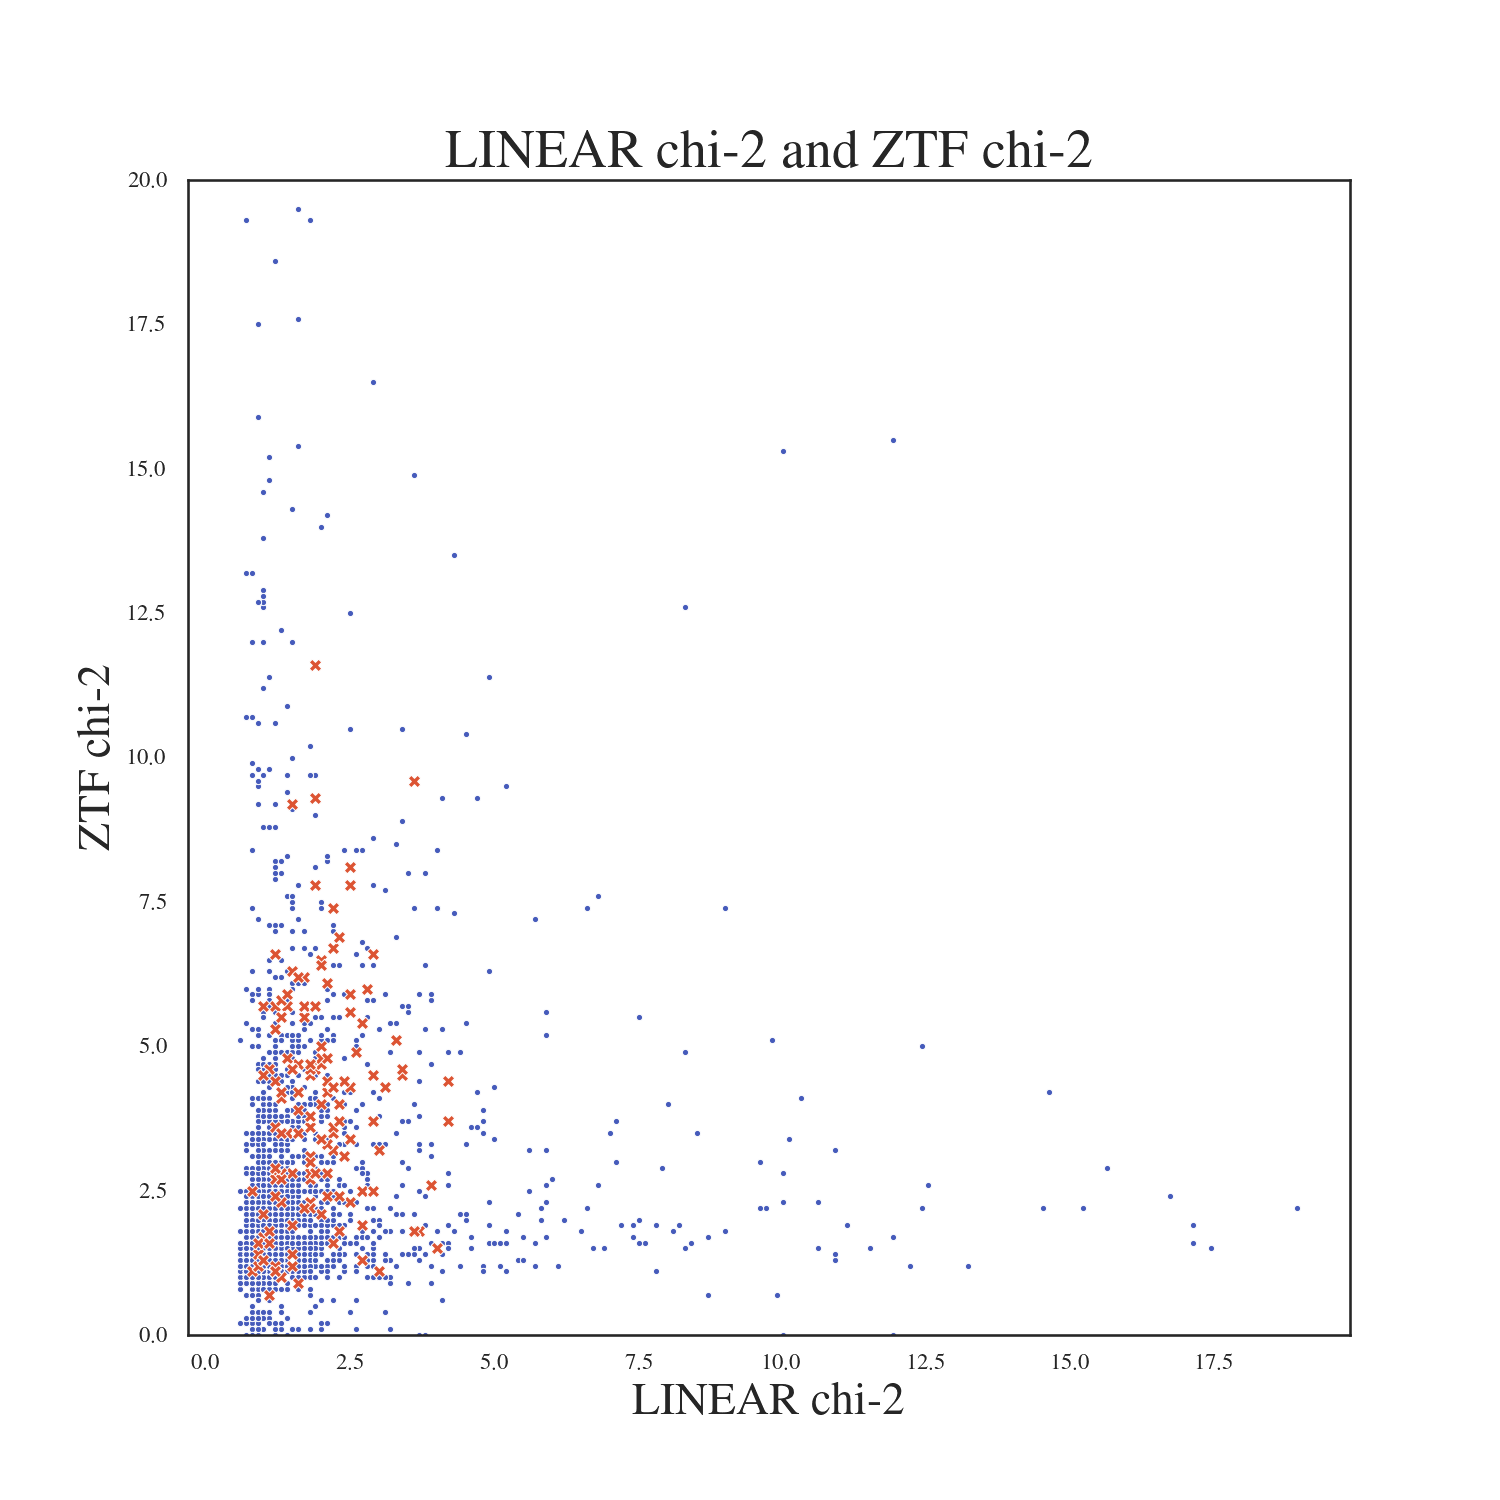
\includegraphics{chi_scatter.png}}
\caption{$\chi^2$ values for LINEAR and ZTF, where blue are all RR Lyrae stars and red are Blazhko stars.}
\label{fig:chi2}
\end{figure}

Another important note highlighting the difficulty of finding Blazhko stars is that the absolute Blazhko frequency difference from the main frequency is approximately 0.028 $d^{-1}$. Also, the average period difference between LINEAR and ZTF in Blazhko stars was around 0.0001 days. These minimal differences require precise observations over a long temporal baseline. The distribution of RRab and RRc type RR Lyrae in our sample is representative of other surveys, where 71\% were type RRab and 29\% RRc type.

Finally, we have discovered that in some Blazhko stars, the effect cannot be detected ten years later or beforehand. When comparing LINEAR and ZTF data, some pairs have the effect present in only one dataset and others in both. This finding could mean that the Blazhko effect is not always present and gives us a clue about its mechanism. However, the precision of data is also a factor for consideration. 

\begin{figure*}[ht]
  \centering
  
\includegraphics[width=17cm]{LCplot_7048826.png}
       \caption{Phase 1 of visual analysis of Blazhko candidates.}
       \label{fig:phase1}
  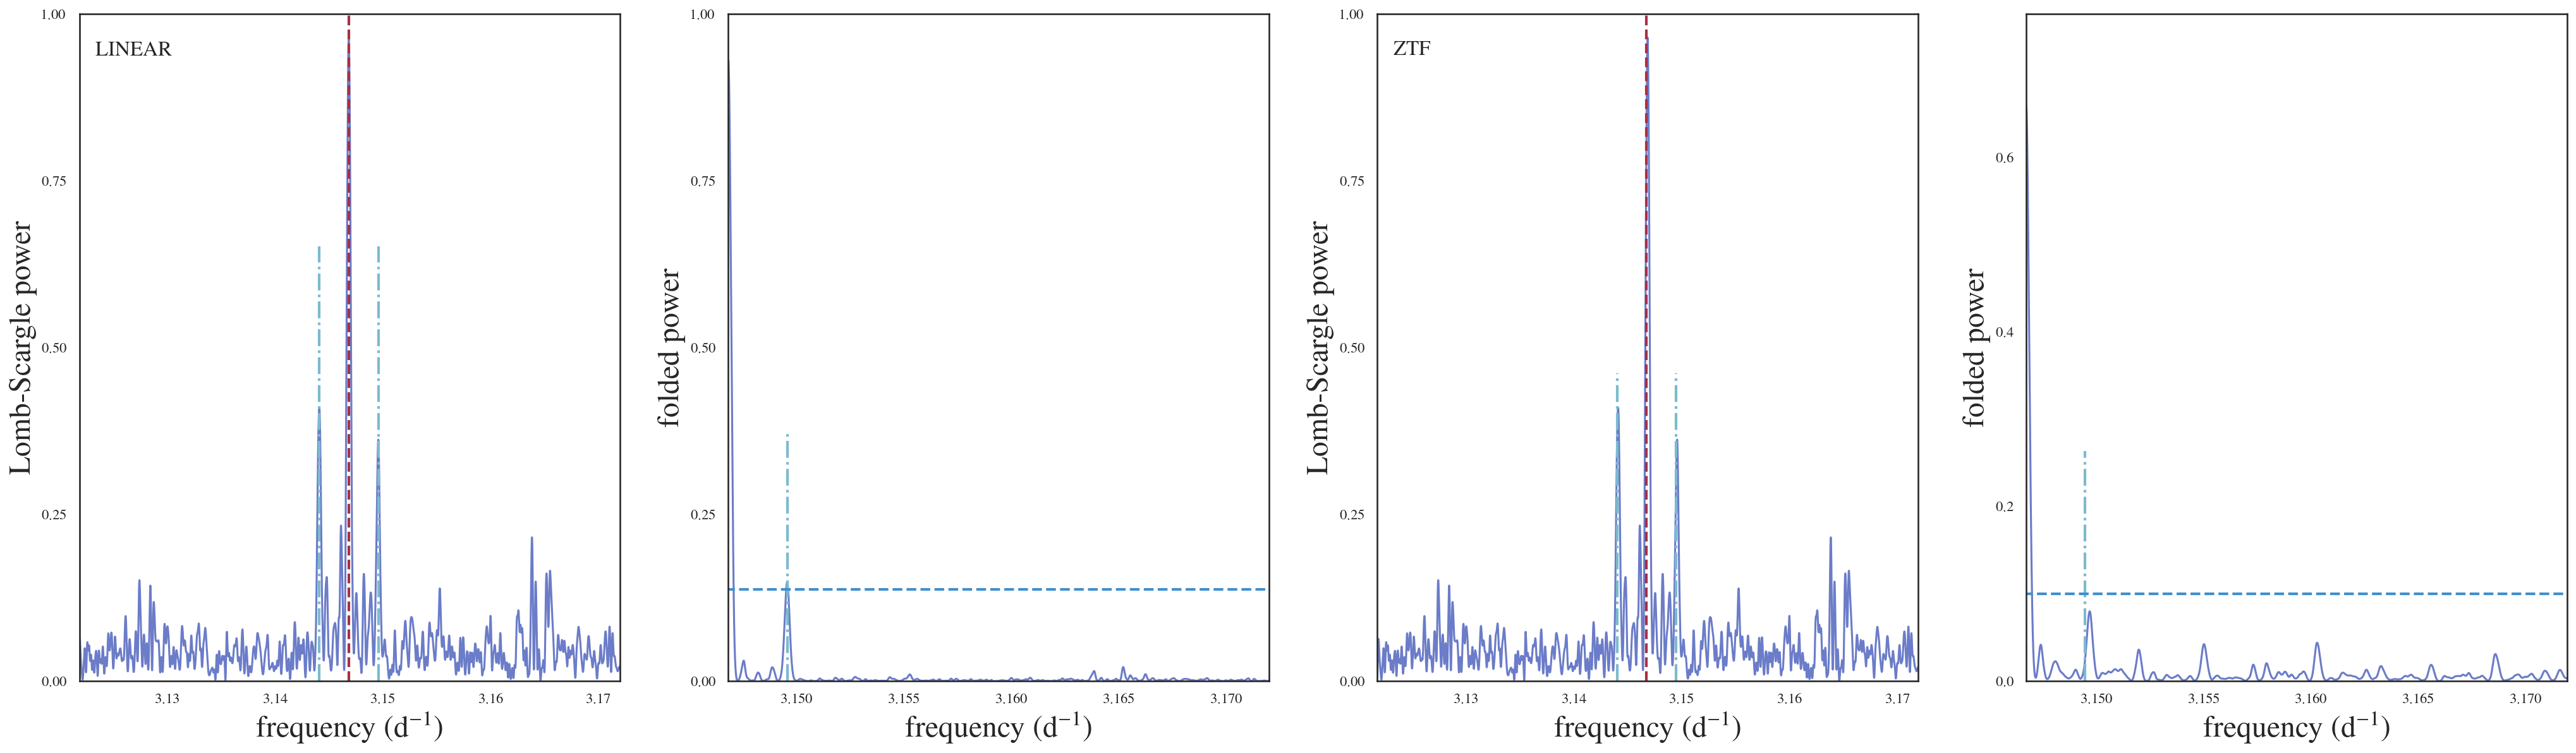
\includegraphics[width=17cm]{periodogram7048826.png}
    \caption{Phase 2 of visual analysis of Blazhko candidates.}
    \label{fig:phase2}

    \centering
       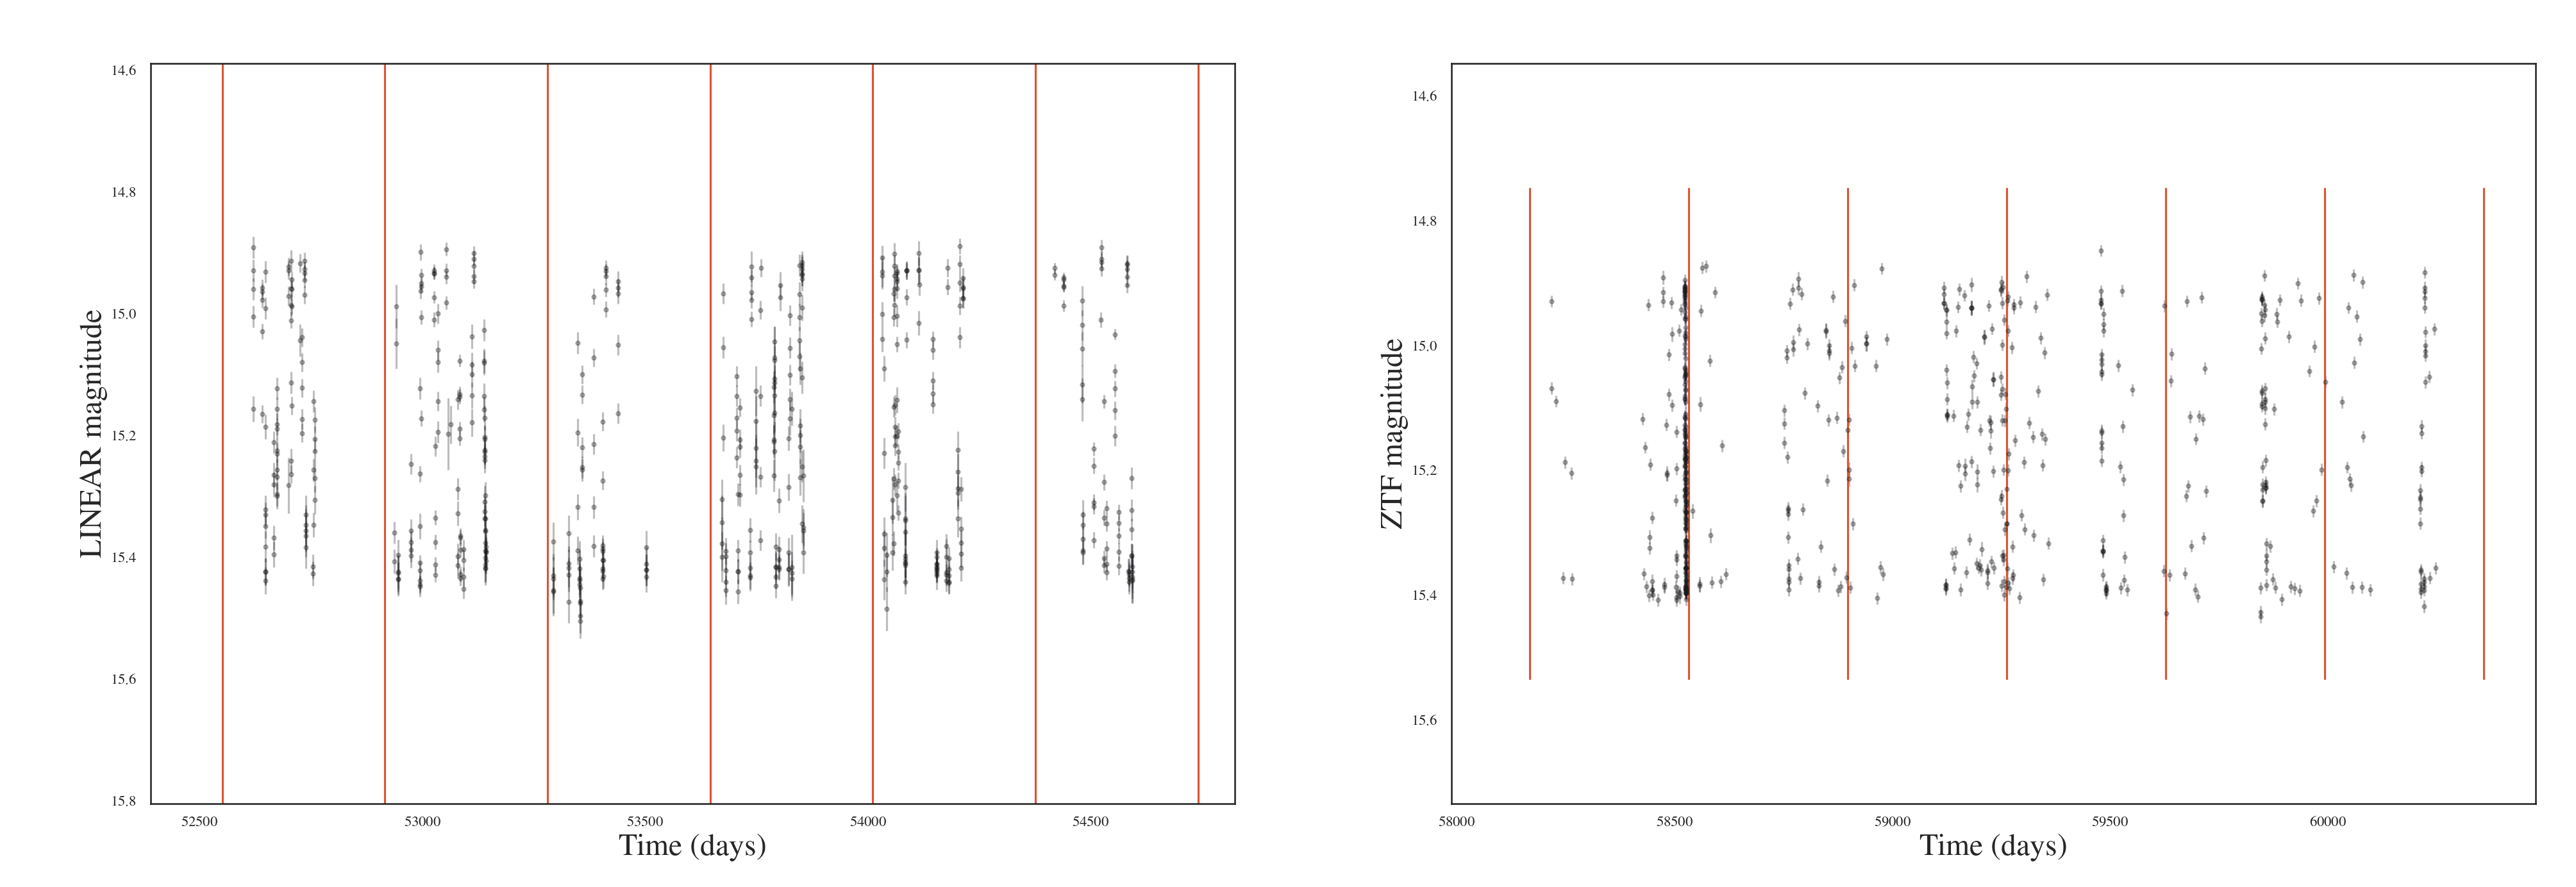
\includegraphics[width=17cm]{season_plot7048826.png}
         \caption{Phase 3 of visual analysis of Blazhko candidates.}
         \label{fig:phase3}
\end{figure*}
\begin{figure*}[ht]
    \centering
    \includegraphics[width=17cm]{LCplotBySeason7048826.png}
      \caption{Phase 4 of visual analysis of Blazhko candidates.}
      \label{fig:phase4}
\end{figure*}
